% =====================================================================
% Uncertainty-Aware Risk-Adjusted Benchmarking of the Fama-French
% Portfolios: Latent Performance, Rank Uncertainty, and the Limits of
% Forecastability.
%
% Self-contained manuscript. Compile with:
%   latexmk -pdf paper.tex        (or pdflatex paper.tex, run twice)
% Depends only on packages shipped with a minimal TeX Live / TinyTeX:
%   geometry, amsmath, amssymb, booktabs, graphicx, natbib, hyperref.
% Figures are read from ../../results/figures (see \graphicspath).
% Every numerical value is taken from the canonical result tables in
% ../results/tables produced by `python -m analysis.run_all`.
% All references were verified against Crossref; each carries a DOI link.
% =====================================================================
\documentclass[11pt]{article}

\usepackage[T1]{fontenc}
\usepackage{lmodern}
\usepackage[margin=1in]{geometry}
\usepackage{amsmath,amssymb}
\usepackage{booktabs}
\usepackage{graphicx}
\usepackage{natbib}
\usepackage[hidelinks]{hyperref}

\graphicspath{{../../results/figures/}}
\bibpunct{(}{)}{;}{a}{}{,}
\setlength{\parskip}{4pt}

\title{\bfseries Uncertainty-Aware Risk-Adjusted Benchmarking of the
Fama--French Portfolios: Latent Performance, Rank Uncertainty, and the
Limits of Forecastability}
\author{Muhammad Shoaib\thanks{Correspondence: Muhammad.Shoaib@utopi.co.uk.
This paper reports historical research diagnostics on passively constructed
research portfolios. It is not investment advice, a trading strategy, or
evidence of manager-specific skill. All results regenerate from
\texttt{python -m analysis.run\_all}.}}
\date{This version: July 2026}

\begin{document}
\maketitle

\begin{abstract}
\noindent
We benchmark the 25 Fama--French size and book-to-market portfolios on a
validated balanced panel of 29,825 portfolio-months (1,193 months, July
1926--November 2025). The estimand is the Fama--French three-factor (FF3)
alpha; the primary uncertainty object is the full $25\times25$
heteroskedasticity- and autocorrelation-consistent (HAC) covariance of the
alpha vector; and the reported score is a multivariate empirical-Bayes
posterior alpha. Rankings carry common-date block-bootstrap rank intervals and
are evaluated out of sample. The joint HAC/Wald test rejects the hypothesis
that all alphas are zero ($p=6.4\times10^{-10}$), yet partial pooling, wide
bootstrap rank intervals, and strong long-horizon mobility show that the point
ranking is not a precise hierarchy. In strictly forward windows the
top-minus-bottom quintile spread averages 243~bps/year. Our central
contribution is an \emph{incremental} test that decomposes this signal: framed
as a Diebold--Mariano test of equal predictive accuracy, the time-varying
rolling ranking adds no power over a leakage-free expanding-window ranking
(mean skill differential $-0.042$, HAC $t=-1.87$) and is dominated by a single
fixed full-sample ordering. The forward result is therefore consistent with
persistent characteristic mispricing, not dynamic forecasting skill. Alpha is
benchmark-dependent (an 11-rank FF3-to-FF5 move), and only one of 25
stochastic-frontier boundary tests survives false-discovery control. The
findings extend the skeptical and out-of-sample asset-pricing literatures to
the question of whether \emph{re-estimating} a cross-sectional ranking through
time is worthwhile; here it is not.
\end{abstract}

\noindent\textbf{Keywords:} cross-sectional asset pricing; empirical Bayes;
HAC inference; rank uncertainty; out-of-sample validation; predictive
accuracy; false-discovery control.\\
\textbf{JEL classification:} G11, G12, C11, C58.

% =====================================================================
\section{Introduction}
% =====================================================================
A portfolio can earn a high average return because it bears systematic risk,
because its sample happened to be favourable, because the benchmark is
incomplete, or because it contains genuinely unusual performance. Factor
benchmarking removes the part linearly associated with priced factors and
studies the intercept, or alpha. For the 25 Fama--French portfolios---the
canonical test assets from which the size and value factors are built
\citep{FamaFrench1993}---this intercept is a model-relative quantity: it is
unexplained by the chosen factors, not by every conceivable risk or friction.

This paper makes the uncertainty around such a benchmark explicit and then
asks a sharper question than the usual out-of-sample test. Our contributions
are fourfold. First, we estimate the full cross-portfolio HAC covariance of
the 25 alphas \citep{NeweyWest1987} rather than 25 unrelated standard errors,
and use it for the joint test of \citet{GRS1989} and for multivariate
empirical-Bayes shrinkage \citep{EfronMorris1973}. Second, we quantify ranking
uncertainty with a common-date circular block bootstrap
\citep{Kunsch1989,PolitisRomano1994} that refits every stage of the estimator.
Third, we separate description from validation with a strictly forward
evaluation in which scores, ranks, and factor loadings are frozen before the
evaluation window. Fourth---and centrally---we introduce an \emph{incremental}
forward test that isolates whether the time-varying ranking adds anything
beyond a fixed characteristic ordering. We show that this test is a
Diebold--Mariano test of equal predictive accuracy \citep{DieboldMariano1995},
with the \citet{GiacominiWhite2006} interpretation for rolling estimation
schemes.

The headline results are as follows. The joint zero-alpha hypothesis is
rejected under the dependence-robust HAC/Wald test, and five of 25 individual
alphas survive 5\% Benjamini--Hochberg false-discovery control
\citep{BenjaminiHochberg1995}. Yet bootstrap rank intervals are wide and
long-horizon quintile mobility is high, so the point ranking is not a reliable
league table---an outcome anticipated by \citet{LewellenNagelShanken2010}. The
strictly forward top-minus-bottom quintile spread is positive on average
(243~bps/year). The incremental test then shows that this predictability is
\emph{not} dynamic: the 120-month rolling ranking beats a naive size/value
characteristic gradient but does not beat a leakage-free expanding-window
ranking, and is itself dominated by a single fixed full-sample ordering. The
predictive content lives in a stable, irregular cross-sectional alpha pattern
that FF3 misprices persistently, not in the re-estimation of the ranking
through time. This mirrors, in the cross-section, the fragility of adaptive
out-of-sample prediction documented by \citet{WelchGoyal2008} and the
characteristic-based, decaying nature of anomaly returns in
\citet{McLeanPontiff2016}.

The remainder of the paper is organised as follows. Section~\ref{sec:lit}
reviews the related literature. Section~\ref{sec:data} describes the data and
integrity checks. Section~\ref{sec:method} sets out the estimator.
Section~\ref{sec:results} reports the empirical results, Section~\ref{sec:robust}
the robustness and validation analysis, Section~\ref{sec:discussion} discusses
interpretation, and Section~\ref{sec:conclusion} concludes.

% =====================================================================
\section{Related literature}\label{sec:lit}
% =====================================================================
\paragraph{Factor benchmarking and test assets.}
\citet{FamaFrench1993} introduced the three-factor model and the 25 size and
book-to-market portfolios that remain the standard test assets, and
\citet{GRS1989} provided the finite-sample joint test that all intercepts are
zero. \citet{FamaFrench2015} added profitability and investment factors, and
\citet{FamaFrench2016} document that the model's most serious pricing failures
involve the smallest, lowest-book-to-market stocks---the ``small-growth''
cell. \citet{Cochrane2011} reframes asset pricing around cross-sectional
variation in expected returns. Our paper benchmarks exactly these test assets
and reproduces the small-growth shortfall as the lowest-ranked cell.

\paragraph{Skepticism about alphas and cross-sectional tests.}
\citet{LewellenNagelShanken2010} show that high cross-sectional fit and large
apparent alphas on size/book-to-market portfolios can be misleadingly strong,
and recommend stricter standards, confidence intervals, and attention to the
factor structure of the test assets. \citet{HarveyLiuZhu2016} argue that the
proliferation of candidate factors demands higher significance hurdles and
multiple-testing corrections. These concerns motivate our use of the full
joint HAC covariance, Benjamini--Hochberg false-discovery control, and
bootstrap rank intervals rather than isolated $t$-statistics.

\paragraph{Shrinkage and empirical Bayes.}
The winner's curse in ranking noisy estimates is classically addressed by
Stein-type shrinkage and empirical Bayes \citep{EfronMorris1973}, applied to
portfolio problems by \citet{Jorion1986}. Recent work shrinks the
cross-section more aggressively---\citet{KozakNagelSantosh2020} on the pricing
kernel and \citet{GuKellyXiu2020} via machine learning---and finds that
disciplined shrinkage and rich conditioning improve out-of-sample
cross-sectional pricing. We use multivariate empirical Bayes with the full
sampling covariance to temper extreme estimates; our negative dynamic result
(below) concerns the time-variation of a coarse 25-cell ranking, not the value
of conditioning information per se, so it does not contradict this literature.

\paragraph{Out-of-sample predictability and its fragility.}
\citet{WelchGoyal2008} show that many equity-premium predictors fail to beat
the historical mean out of sample and that adaptively estimated models often
underperform simple benchmarks. \citet{McLeanPontiff2016} find that anomaly
returns are characteristic-based and decline substantially after publication.
Our incremental finding---a stable ordering predicts future alpha while
dynamic re-estimation does not---is a cross-sectional analogue of both: the
signal is a persistent property of fixed characteristic cells, and chasing it
with a rolling window adds estimation noise rather than information.

\paragraph{Forecast evaluation and bootstrap inference.}
\citet{DieboldMariano1995} test equal predictive accuracy via the mean loss
differential with HAC standard errors, and \citet{GiacominiWhite2006} extend
this to models estimated on rolling windows. We cast the incremental test in
exactly this framework. For finite-sample performance inference we follow the
resampling tradition of \citet{KosowskiTimmermannWermersWhite2006} and
\citet{FamaFrench2010}, using the block bootstrap of \citet{Kunsch1989} and
\citet{PolitisRomano1994} in a common-date, circular form; dependence-robust
covariances follow \citet{NeweyWest1987} with the automatic bandwidth of
\citet{NeweyWest1994}. The secondary residual-asymmetry diagnostic uses the
stochastic-frontier model of \citet{AignerLovellSchmidt1977} with the
conditional-inefficiency estimator of \citet{JondrowLovellMaterovSchmidt1982}.

\paragraph{Contribution.}
Prior work either tests the alpha vector jointly \citep{GRS1989} or evaluates a
cross-sectional ranking out of sample. We add a decomposition that separates
the \emph{dynamic} content of a re-estimated ranking from the \emph{static}
content of a fixed ordering, and show---using a Diebold--Mariano/Giacomini--White
test on strictly forward data---that the dynamic component is statistically
indistinguishable from zero for the 25 Fama--French portfolios.

% =====================================================================
\section{Data}\label{sec:data}
% =====================================================================
\subsection{Portfolios and sample}
The 25 test portfolios form a $5\times5$ grid. At each formation date eligible
stocks are sorted independently into five size and five book-to-market groups;
returns within each of the 25 intersections are value weighted. Labels such as
\textsc{small hibm} and \textsc{big lobm} describe the two sorting dimensions,
not individual firms or managed funds. The unit of observation is one
portfolio-month; the dependent variable is the portfolio return minus the
one-month risk-free rate, $y_{it}=r_{it}-r_{ft}$, in decimal monthly units. The
canonical benchmark is FF3 (Mkt$-$RF, SMB, HML). Annualised basis points
multiply monthly decimal alpha by $12\times10{,}000$, a linear reporting
convention. The validated balanced panel has 29,825 portfolio-months over
1,193 consecutive months (July 1926--November 2025), with zero duplicate keys
and no missing calendar months; the loader fails closed on any violation.

\subsection{Integrity and provenance}
Each run records the SHA-256 digest and byte count of both inputs. A current
(May 2026) official snapshot from the Kenneth R.\ French Data Library is
retained separately and never overwrites the fixed local inputs. The local
sample's exact acquisition vintage is unverified, and the two sources differ
over their overlap---by up to 1.4167 percentage points for portfolio returns
and 0.34 percentage points for FF3/RF fields. Official historical revisions are
a plausible but unproven cause. Both comparisons are therefore classified
\textsc{not\_comparable} (visible, non-blocking) rather than \textsc{pass}.
This is a genuine limitation: the headline numbers rest on inputs that cannot
currently be reconstructed byte-for-byte from the public source, even though all
within-pipeline integrity and independent-replication checks pass
(Section~\ref{sec:robust}).

% =====================================================================
\section{Methodology}\label{sec:method}
% =====================================================================
\subsection{Factor model and the meaning of alpha}
For portfolio $i$ in month $t$, the benchmark regression is
\begin{equation}
y_{it}=\alpha_i+\beta_i'f_t+\varepsilon_{it},
\end{equation}
where $f_t$ stacks the FF3 factor returns and $\alpha_i$ is the mean excess
return left after the fitted linear factor component is removed. Ordinary least
squares gives $\hat\theta_i=(X'X)^{-1}X'y_i$; selecting the intercept, the
estimation error is a weighted sum of residual shocks,
$\hat\alpha_i-\alpha_i=\sum_t a_t\varepsilon_{it}$, where the scalar weight
$a_t$ depends only on the common factor design. Because every portfolio shares
the same dates and factors, these weights combine with the same-month residual
vector to yield a \emph{joint} covariance. A positive alpha denotes in-sample
benchmark-relative outperformance, not skill or future profit; a negative alpha
can reflect omitted risk rather than inefficiency.

\subsection{Full joint HAC covariance}
Let $e_t$ be the 25-vector of same-month residuals and $g_t=a_t e_t$ the alpha
score vector. With $L=12$ lags, Bartlett weights $w_l=1-l/(L+1)$, and lag-$l$
cross-product $\Gamma_l=\sum_{t>l} g_t g_{t-l}'$, the covariance is
\begin{equation}
V_{\mathrm{HAC}}=\frac{T}{T-P}\Big\{\Gamma_0+\sum_{l=1}^{L} w_l(\Gamma_l+\Gamma_l')\Big\},
\end{equation}
with $P=K+1$ regression coefficients \citep{NeweyWest1987}. This $25\times25$
matrix keeps individual alpha variances on its diagonal and cross-portfolio
co-movement off-diagonal. The implementation symmetrises the result, checks
eigenvalues, and permits only scale-relative flooring of negligible numerical
negatives. The canonical matrix is positive definite without flooring, with
condition number 139.4.

\subsection{Multivariate empirical Bayes}
Ranking 25 noisy estimates invites a winner's curse. Partial pooling treats the
latent alphas as one cross-section,
\begin{equation}
\hat\alpha\mid\alpha\sim N(\alpha,V_{\mathrm{HAC}}),\qquad
\alpha\sim N(\mu\mathbf{1},\tau^2 I),
\end{equation}
with posterior mean
$\mu\mathbf{1}+\tau^2(V_{\mathrm{HAC}}+\tau^2 I)^{-1}(\hat\alpha-\mu\mathbf{1})$
and conditional covariance
$\tau^2 I-\tau^4(V_{\mathrm{HAC}}+\tau^2 I)^{-1}$. The hyperparameters
$(\mu,\tau)$ are estimated by profile marginal maximum likelihood, so the prior
is learned from the same cross-section \citep{EfronMorris1973,Jorion1986}. The
fitted prior mean is $-26$~bps/year with dispersion 94~bps/year. Reported
intervals include first-order uncertainty in the profiled mean but do not fully
integrate uncertainty in $\tau$, and the HAC covariance is treated as known;
the intervals are therefore mildly optimistic model-based summaries.

\subsection{Joint and multiple testing}
The primary joint test is the dependence-robust Wald statistic
$W=\hat\alpha' V_{\mathrm{HAC}}^{-1}\hat\alpha\sim\chi^2(25)$ under the null
that all alphas are zero. The \citet{GRS1989} $F$-test is reported as a
conventional secondary benchmark; its exact reference assumes IID Gaussian
errors, which the diagnostics reject (Section~\ref{sec:robust}). Individual
raw-alpha $p$-values and the 25 stochastic-frontier boundary $p$-values form
two separate Benjamini--Hochberg families \citep{BenjaminiHochberg1995}, since
they test different nulls.

\subsection{Bootstrap rank uncertainty}
A rank is discontinuous, so individual standard errors do not describe how often
a portfolio stays in the top five. We draw 5,000 circular 12-month blocks of
common date indices \citep{Kunsch1989,PolitisRomano1994}, apply the same dates
to all 25 portfolios (preserving cross-sectional shocks), and refit the
regressions, the full HAC covariance, and the empirical-Bayes hyperparameters
within every replicate before re-ranking. Rank and score intervals are
empirical 2.5--97.5\% quantiles of this resampling distribution.

\subsection{Forward validation and the incremental test}\label{sec:incmethod}
For each 120-month training window we freeze all scores, ranks, prior
parameters, and betas at the cutoff, then compute each portfolio's next
12-month benchmark-adjusted return with the frozen loadings,
$A_i^{+}=\overline{y_{it}-\hat\beta_i'f_t}$. Within each evaluation year we
compute the Spearman correlation between training scores and future alpha and
the average top-minus-bottom quintile spread; annual statistics are aggregated
with a Fisher transformation and four-lag HAC inference. Evaluation windows do
not overlap.

The forward test alone cannot separate genuine dynamic skill from persistent
characteristic mispricing: because FF3 misprices fixed characteristic cells in a
stable way, a ranking anchored to past alpha will correlate with future alpha
mechanically. We therefore add an \emph{incremental} test that scores the
rolling ranking against a competing benchmark ordering on the \emph{same}
forward observations. For window $j$ let $d_j$ be the difference between the
rolling ranking's predictive score (Spearman correlation with future alpha, or
the quintile spread) and the benchmark's. The mean differential $\bar d$ with a
HAC standard error is exactly the \citet{DieboldMariano1995} test of equal
predictive accuracy, and because the competing rankings are re-estimated on
rolling/expanding schemes it carries the \citet{GiacominiWhite2006}
interpretation. We use four benchmark orderings: (i) a size-ascending,
book-to-market-descending characteristic gradient; (ii) a diagonal
value-minus-size gradient; (iii) a leakage-free \emph{expanding-window} ranking
re-estimated on all data up to each cutoff; and (iv) a full-sample \emph{oracle}
ordering, which uses look-ahead information and is thus an upper bound on what a
static ranking can achieve. Benchmark (iii) is the fair, tradable comparator on
which the interpretation rests. The per-window differential is aggregated with
an automatic-bandwidth Newey--West HAC $t$-test \citep{NeweyWest1994} and a
block bootstrap.

% =====================================================================
\section{Results}\label{sec:results}
% =====================================================================
\subsection{Cross-sectional posterior performance}
Table~\ref{tab:ranking} reports the full ranking. \textsc{small hibm} has the
highest posterior alpha (132~bps/year) and \textsc{small lobm} the lowest
($-185$~bps/year), reproducing the well-known small-value premium and
small-growth shortfall relative to FF3 \citep{FamaFrench2016}. Two posterior
intervals are wholly above zero (\textsc{small hibm}, \textsc{big lobm}); most
cross zero. Five raw-alpha tests survive Benjamini--Hochberg control, but four
of these correspond to significantly negative alpha, so raw-test significance
and posterior rank are distinct summaries.

\begin{table}[htbp]
\centering
\caption{Posterior FF3 performance ranking (annualised basis points). Raw and
posterior alpha in bps/year; posterior 95\% is the empirical-Bayes interval;
BH $q$ is the false-discovery-adjusted raw-alpha $p$-value; the bootstrap rank
interval is the central 95\% range over 5,000 common-date circular-block
draws.}
\label{tab:ranking}
\small
\begin{tabular}{r l r r c c c}
\toprule
Rank & Portfolio & Raw $\alpha$ & Post.\ $\alpha$ & Post.\ 95\% & BH $q$ & Boot.\ rank 95\% \\
\midrule
1 & SMALL HiBM & 169 & 132 & [23, 240] & 0.063 & [1.0, 6.0] \\
2 & BIG LoBM & 118 & 79 & [9, 148] & 0.033 & [1.0, 10.0] \\
3 & ME4 BM1 & 50 & 78 & [-24, 180] & 0.732 & [1.0, 15.0] \\
4 & ME1 BM4 & 84 & 61 & [-47, 169] & 0.456 & [1.0, 12.0] \\
5 & ME3 BM2 & 103 & 55 & [-43, 153] & 0.227 & [1.0, 12.0] \\
6 & ME2 BM5 & 37 & 46 & [-49, 141] & 0.766 & [2.0, 15.0] \\
7 & ME4 BM4 & 23 & 21 & [-83, 125] & 0.861 & [2.0, 18.0] \\
8 & ME2 BM2 & 21 & 16 & [-92, 125] & 0.868 & [2.0, 18.0] \\
9 & ME3 BM4 & 44 & 14 & [-80, 107] & 0.732 & [3.0, 18.0] \\
10 & ME5 BM3 & -38 & 13 & [-95, 121] & 0.825 & [3.0, 19.0] \\
11 & ME2 BM3 & 26 & -7 & [-105, 92] & 0.825 & [3.0, 19.0] \\
12 & ME2 BM4 & 25 & -17 & [-104, 70] & 0.825 & [4.0, 19.0] \\
13 & ME5 BM2 & -5 & -29 & [-112, 55] & 0.912 & [5.0, 20.0] \\
14 & ME4 BM3 & -15 & -29 & [-130, 73] & 0.874 & [6.0, 21.0] \\
15 & ME3 BM3 & 52 & -35 & [-128, 59] & 0.732 & [4.0, 20.0] \\
16 & ME3 BM5 & -76 & -43 & [-155, 68] & 0.562 & [6.0, 22.0] \\
17 & ME4 BM2 & -14 & -77 & [-184, 31] & 0.874 & [9.0, 23.0] \\
18 & BIG HiBM & -198 & -82 & [-229, 65] & 0.336 & [10.0, 24.0] \\
19 & ME3 BM1 & -142 & -82 & [-178, 15] & 0.055 & [11.0, 23.0] \\
20 & ME1 BM3 & -144 & -83 & [-192, 25] & 0.106 & [9.0, 23.0] \\
21 & ME4 BM5 & -211 & -92 & [-218, 35] & 0.063 & [13.0, 24.0] \\
22 & ME1 BM2 & -476 & -115 & [-271, 41] & 0.005 & [15.0, 25.0] \\
23 & ME2 BM1 & -261 & -115 & [-229, -1] & 0.003 & [15.0, 25.0] \\
24 & ME5 BM4 & -289 & -164 & [-268, -60] & 0.002 & [19.0, 25.0] \\
25 & SMALL LoBM & -810 & -185 & [-351, -18] & $<$0.001 & [21.0, 25.0] \\
\bottomrule
\end{tabular}
\end{table}

\begin{figure}[htbp]
\centering
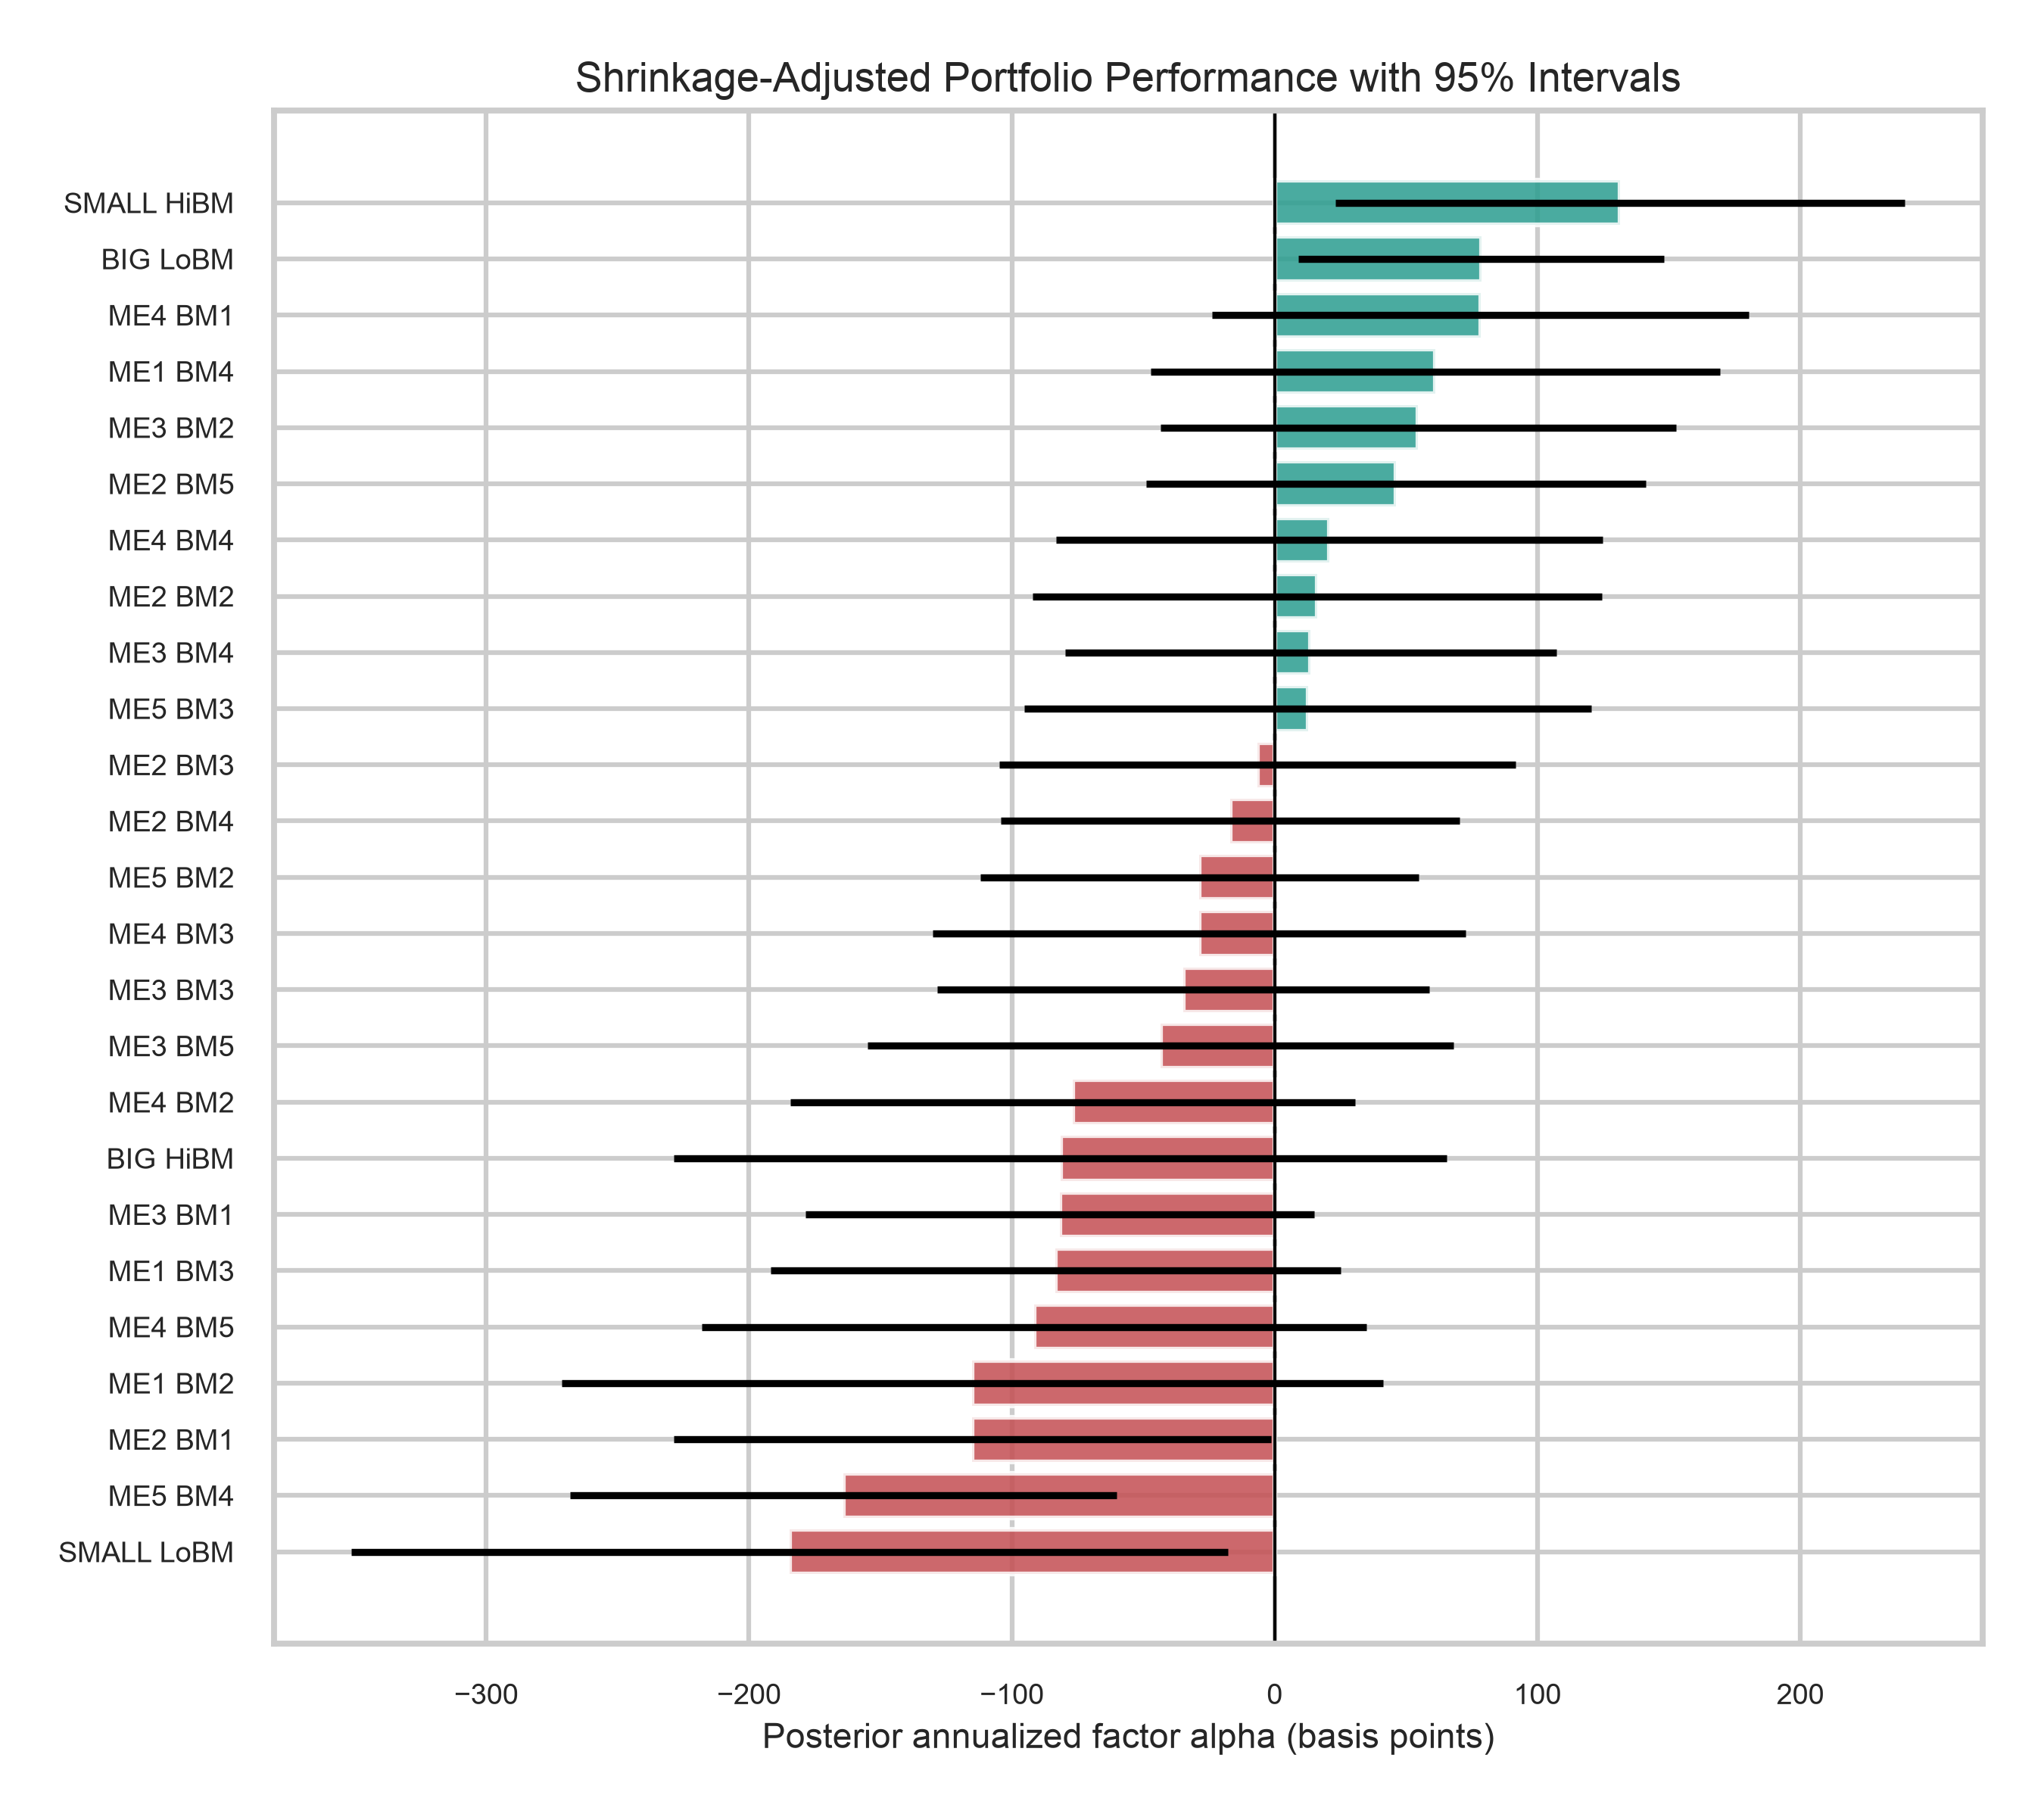
\includegraphics[width=0.72\linewidth]{performance_ranking.png}
\caption{Posterior FF3 alpha (annualised bps) with approximate 95\% posterior
intervals. An interval crossing zero indicates the latent alpha is not cleanly
separated from zero; interval overlap warns that adjacent ranks are not
distinguished.}
\label{fig:ranking}
\end{figure}

\subsection{Joint tests and rank uncertainty}
The HAC/Wald statistic is 93.9 ($p=6.4\times10^{-10}$) and the GRS statistic is
3.28 ($p=1.2\times10^{-7}$); both reject the joint zero-alpha hypothesis, though
the GRS reference is less credible here. Rejection means the 25-dimensional
alpha vector is inconsistent with all-zero under the stated model; it does not
establish that alphas are positive or that the ordering is stable.
Figure~\ref{fig:rankunc} shows the bootstrap rank distribution:
\textsc{small hibm} is rank~1 at the point estimate and in the top quintile in a
majority of resampled histories, yet its central rank interval still reaches
rank~6, and intervals overlap broadly across portfolios. Consistent with
\citet{LewellenNagelShanken2010}, the ordered list is not a precise hierarchy.

\begin{figure}[htbp]
\centering
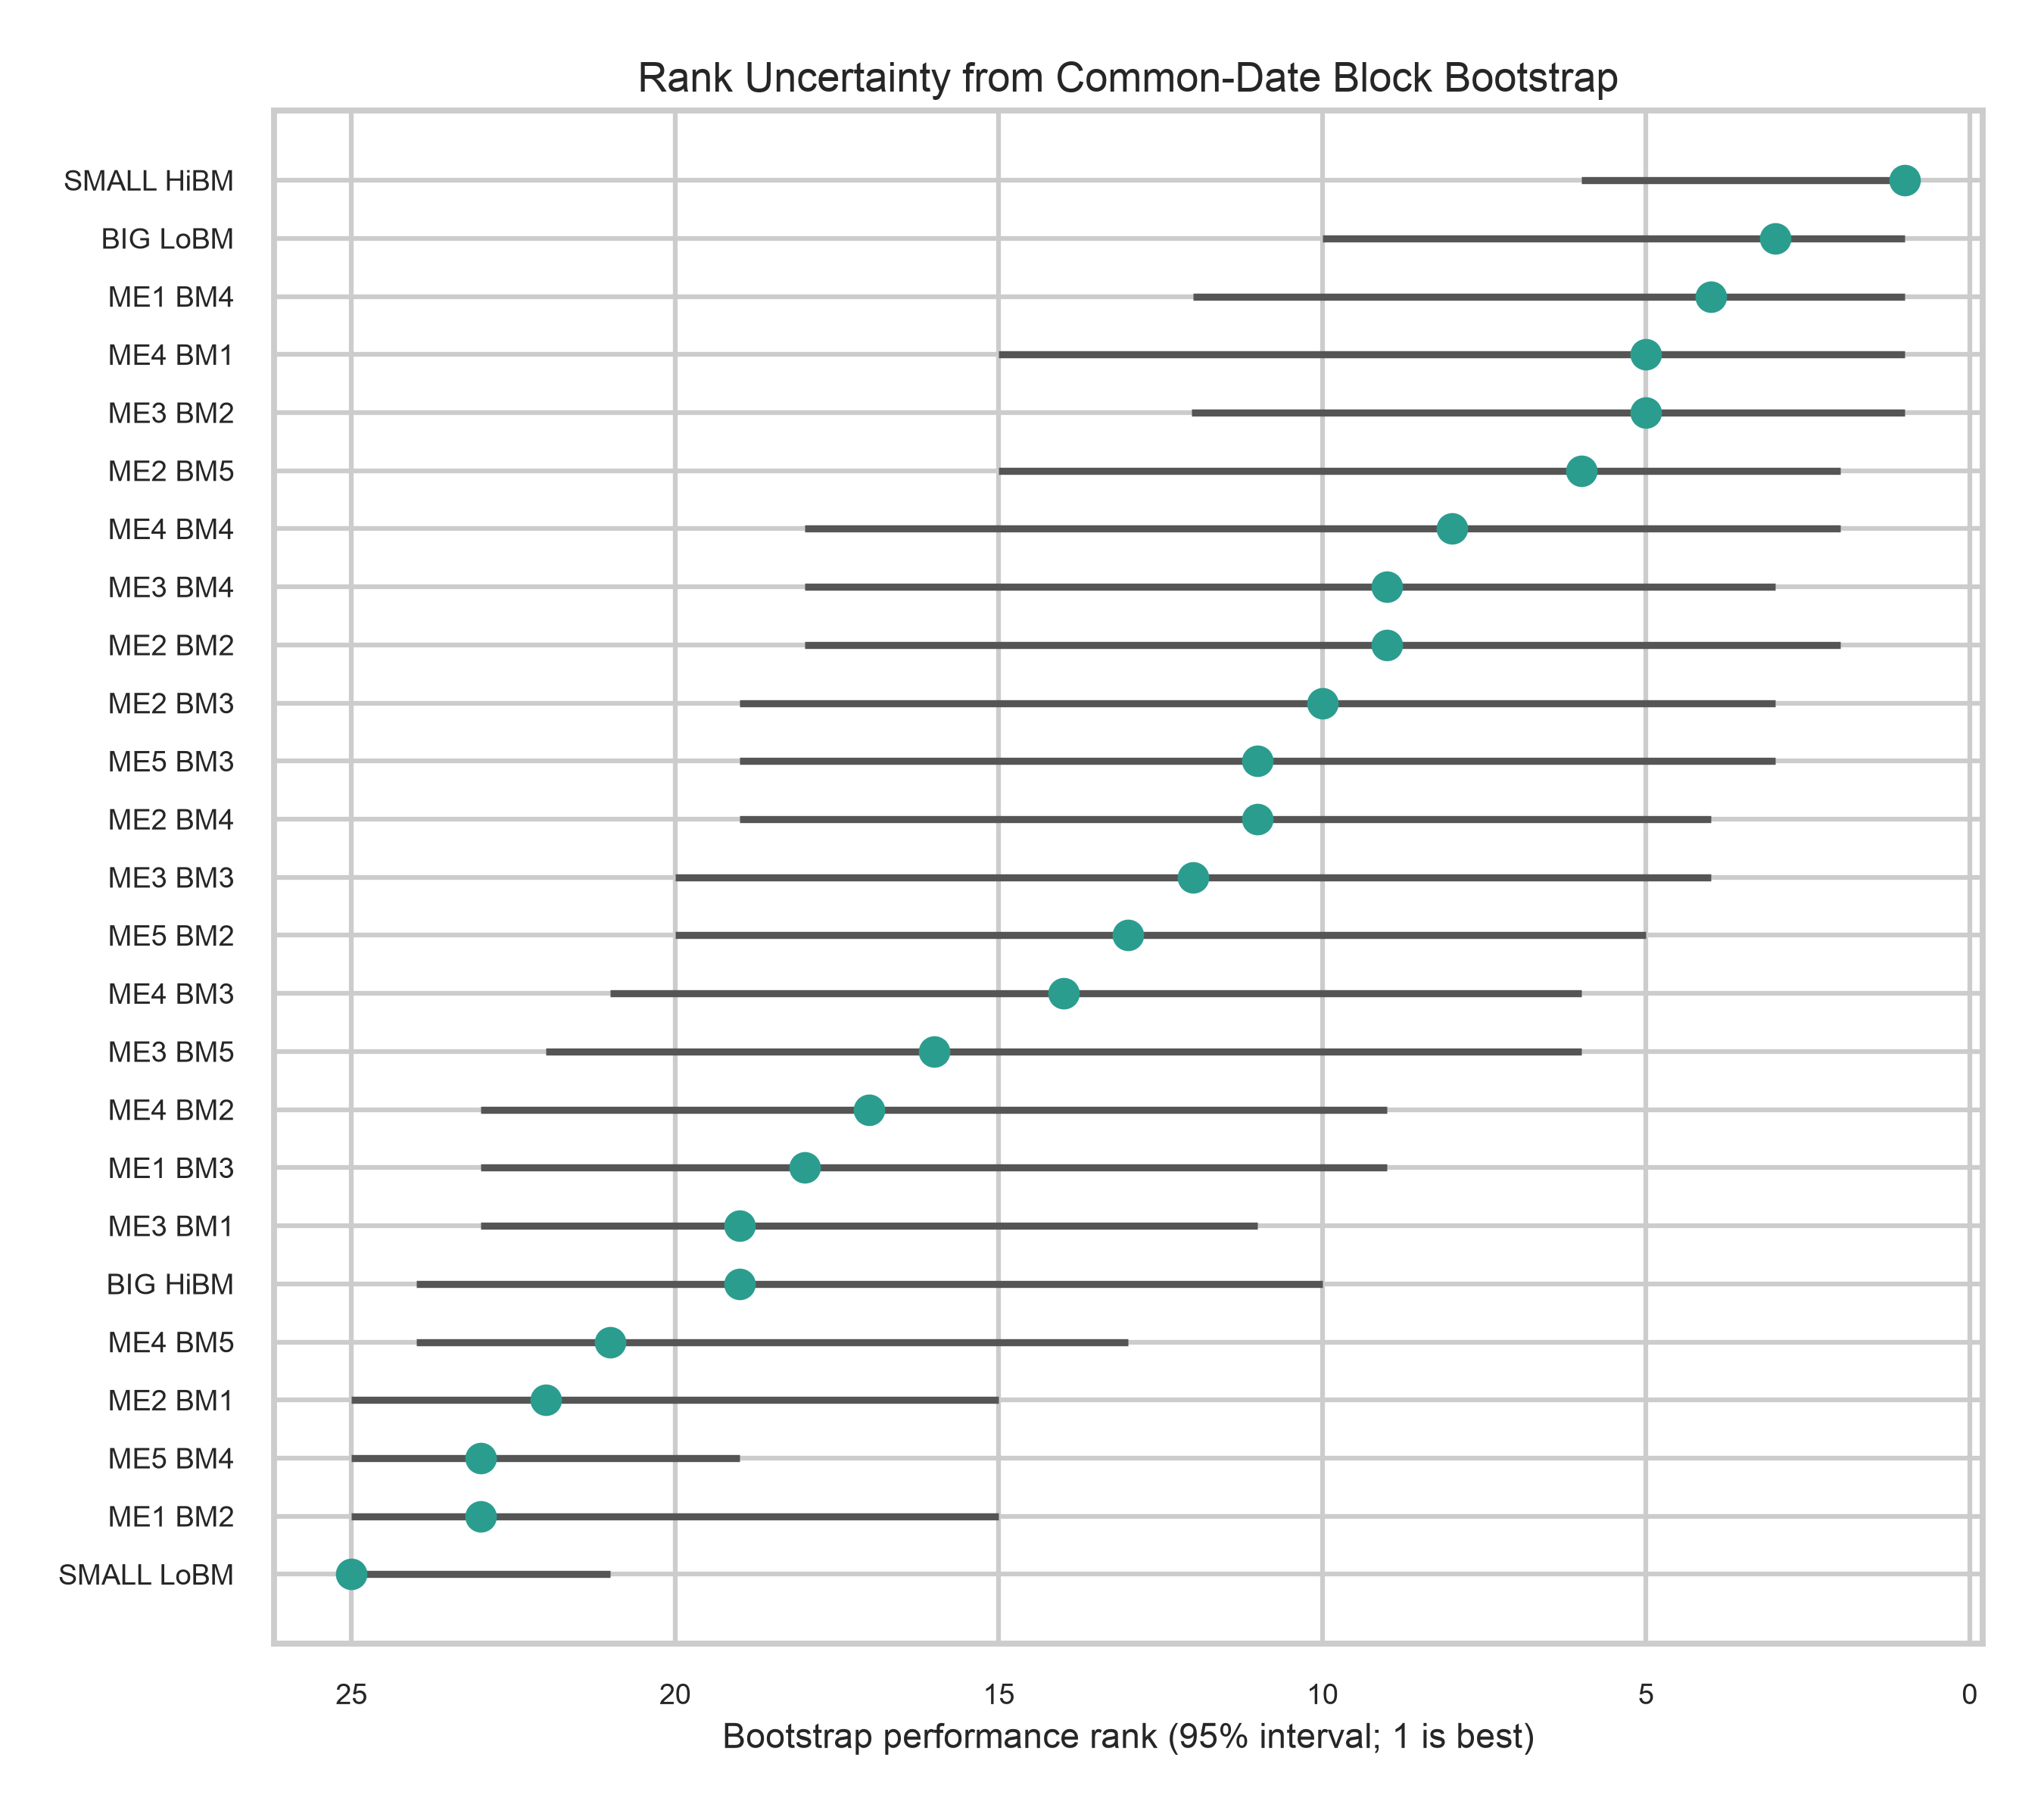
\includegraphics[width=0.72\linewidth]{rank_uncertainty.png}
\caption{Median bootstrap rank and central 95\% rank interval from 5,000
common-date circular-block draws. Broad, overlapping intervals are direct
evidence against reading the ordered list as a precise hierarchy.}
\label{fig:rankunc}
\end{figure}

\subsection{Persistence}
Rank persistence falls from about 0.86 at a 12-month horizon (90\% window
overlap) to roughly 0.16 at 120 months (zero overlap). The non-overlapping
horizon is the credible structural measure and is weak: the mean probability of
staying in the same quintile after 120 months is 24.9\%, essentially the 20\%
implied by uniform mobility. Long-run relative performance is highly mobile.

\subsection{Strictly forward validation}
Across 89 non-overlapping 12-month evaluation periods, the Fisher-averaged rank
correlation between training scores and future alpha is 0.102 (HAC 95\% CI
$[0.055,0.149]$, $p=2.3\times10^{-5}$), and the average top-minus-bottom
quintile spread is 243~bps/year (median 209, IQR 498), positive in 73\% of
windows (Table~\ref{tab:forward}). Both means are statistically distinguishable
from zero, but dispersion across years is large---the IQR exceeds the mean---so
the average is not a uniformly reliable timing rule (Figure~\ref{fig:forward}).

\begin{table}[htbp]
\centering
\caption{Strictly forward validation (four-lag HAC inference), 89
non-overlapping 12-month windows.}
\label{tab:forward}
\small
\begin{tabular}{l r c r}
\toprule
Metric & Estimate & HAC 95\% interval & HAC $p$ \\
\midrule
Rank vs.\ future alpha (Spearman) & 0.102 & $[0.055,\ 0.149]$ & $2.3\times10^{-5}$ \\
Top$-$bottom quintile (bps/year) & 243 & $[153,\ 333]$ & $1.3\times10^{-7}$ \\
\bottomrule
\end{tabular}
\end{table}

\begin{figure}[htbp]
\centering
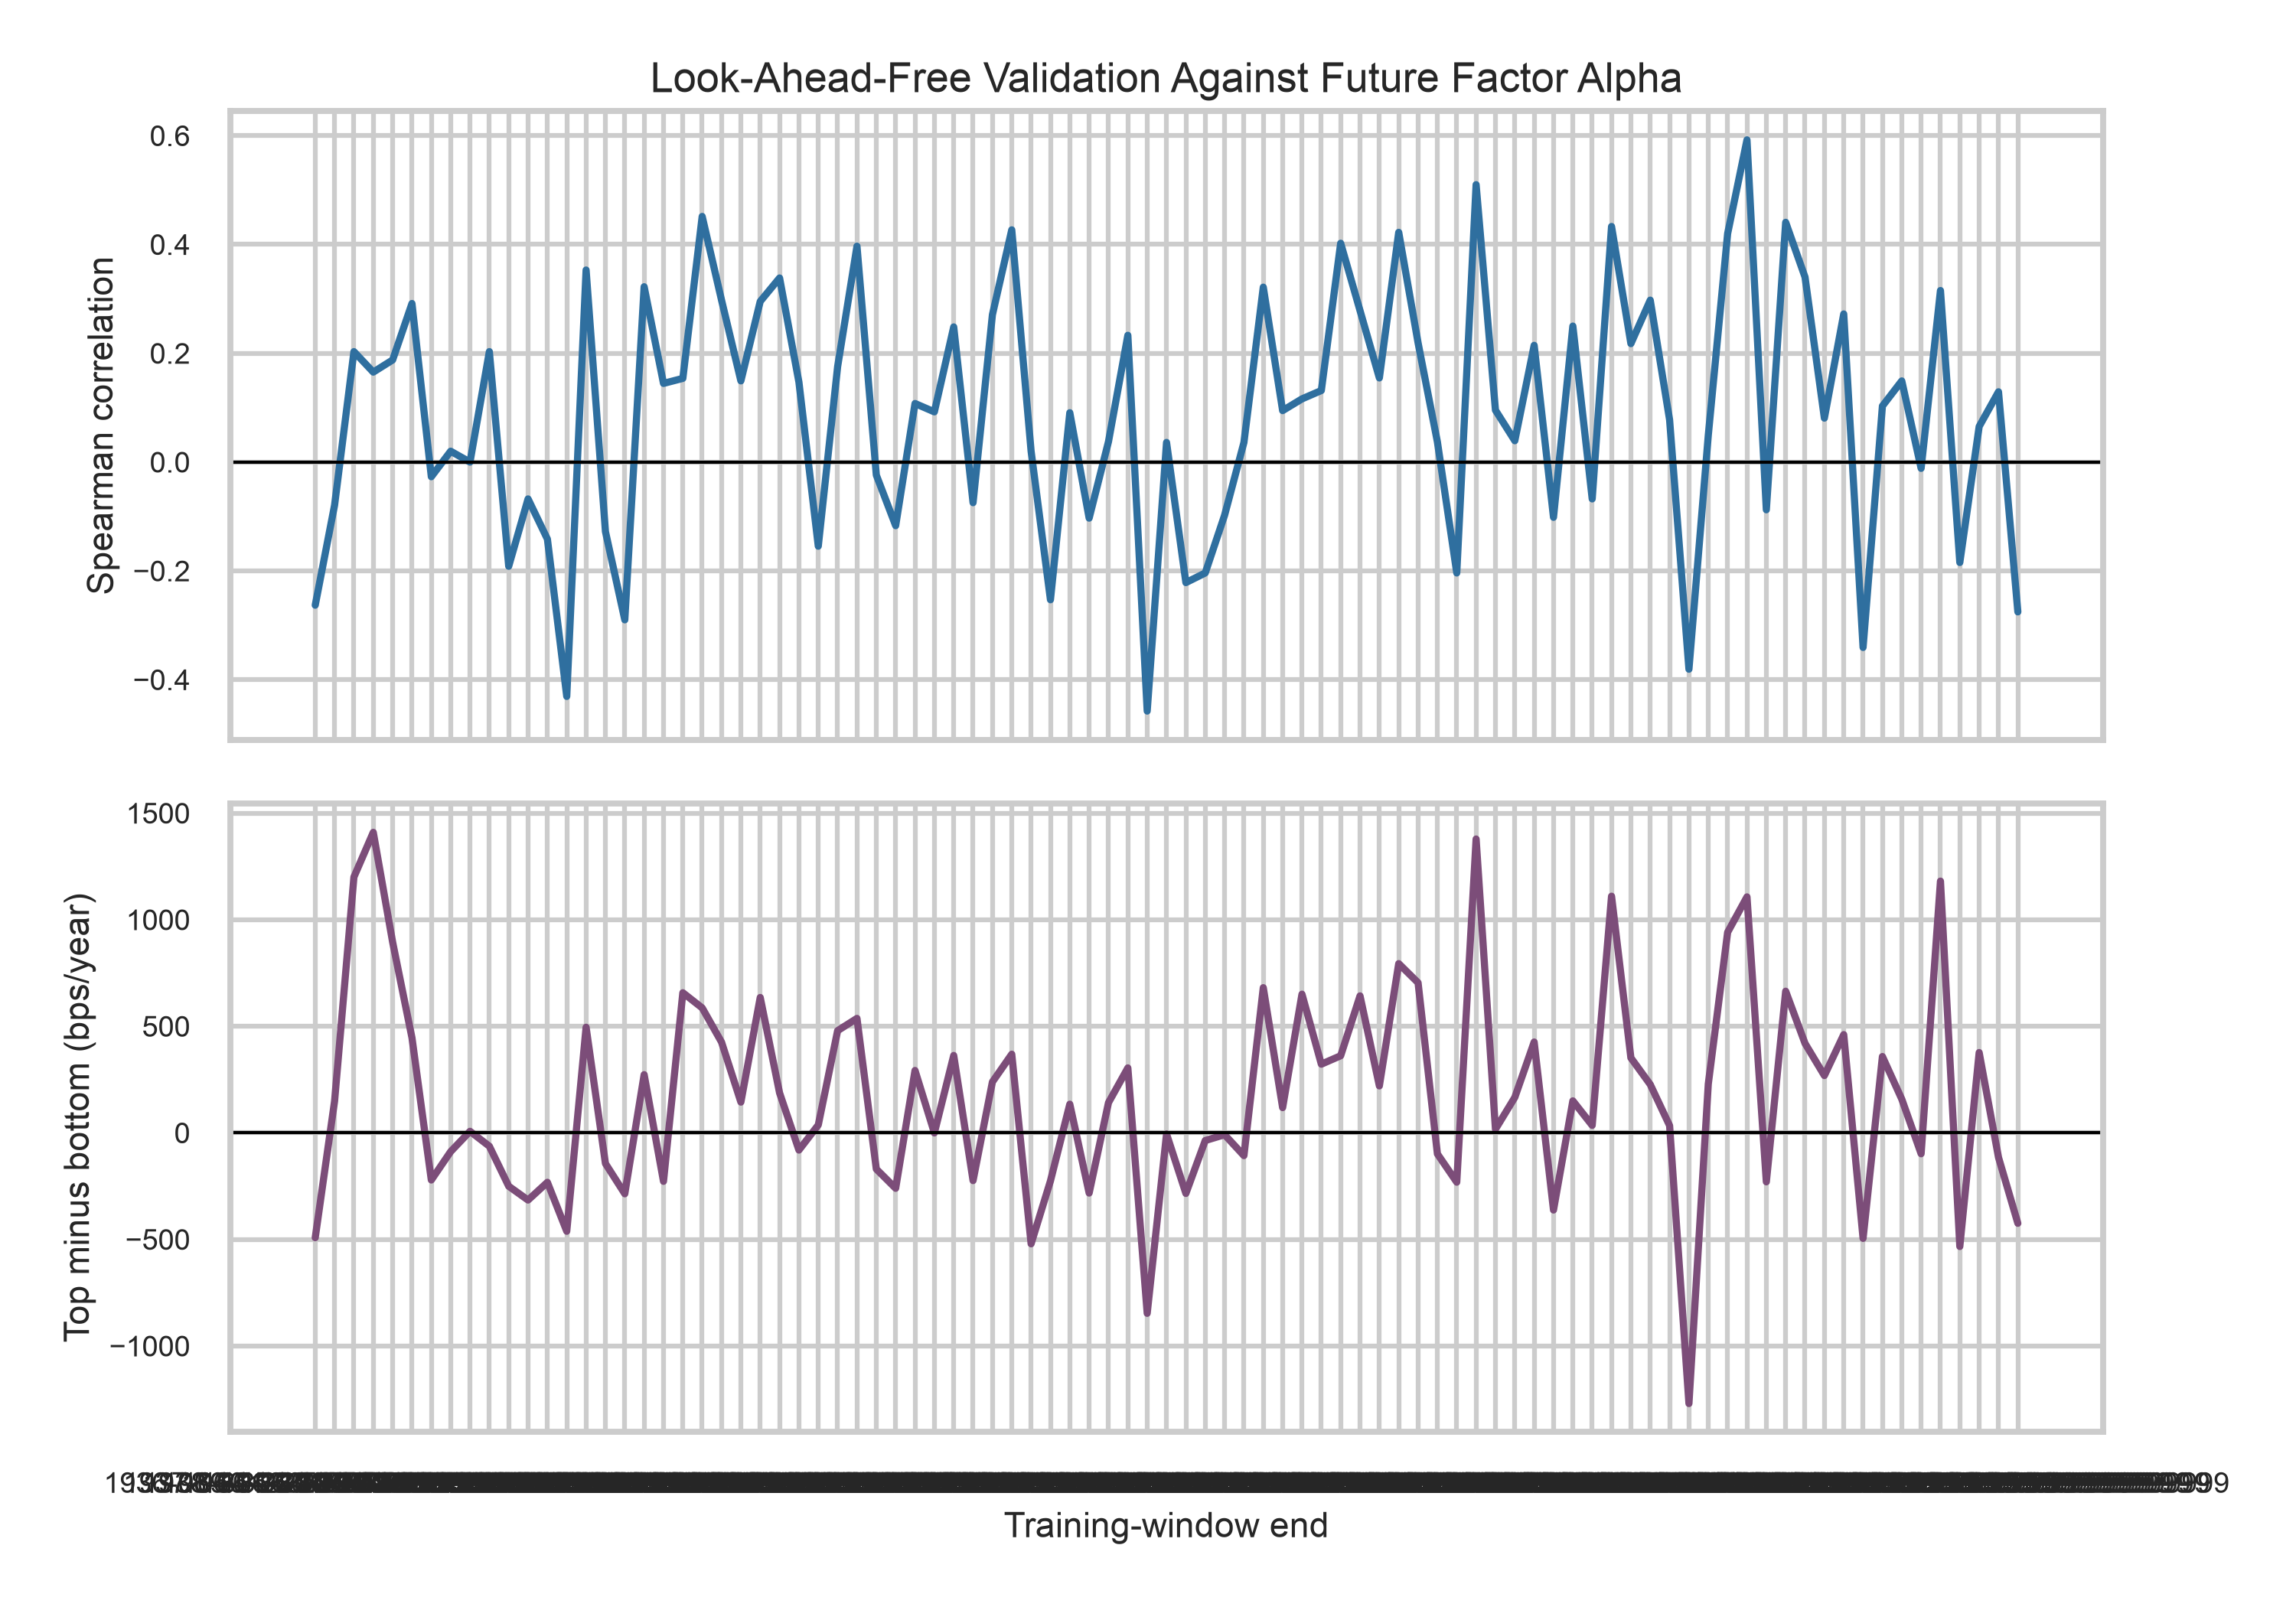
\includegraphics[width=0.82\linewidth]{forward_performance_validation.png}
\caption{Window-by-window future rank correlation (top) and average
top-minus-bottom quintile future alpha (bottom). Frequent negative windows and
large spread variation show the average is not uniformly reliable.}
\label{fig:forward}
\end{figure}

\subsection{The incremental test: is the ranking dynamically informative?}
Table~\ref{tab:incremental} decomposes the forward signal. The rolling ranking's
own level correlation with future alpha is $+0.099$. It exceeds the two static
characteristic gradients---which have essentially zero forward power, because
FF3 alpha is the residual after size and value exposure are removed---so the
rolling signal is not merely a restated size/value tilt. But, read as a
Diebold--Mariano test, it does not beat the leakage-free expanding-window
ranking: the mean skill differential is $-0.042$ with HAC $t=-1.87$ (the block
bootstrap 95\% interval $[-0.085,+0.001]$ includes zero), so we cannot reject
equal predictive accuracy, and the point estimate marginally favours the
expanding benchmark. Against the full-sample oracle the differential is
significantly negative ($-0.100$, $t=-4.18$). A single fixed but irregular
cross-sectional ordering predicts future alpha as well as, or better than, the
ranking that is re-estimated every year (Figure~\ref{fig:incremental}).

\begin{table}[htbp]
\centering
\caption{Incremental predictive power of the rolling ranking versus fixed and
leakage-free benchmarks (Diebold--Mariano equal-predictive-accuracy tests on 89
forward windows; automatic-bandwidth HAC, lag 3). ``Bench.\ corr'' is the
benchmark ordering's own mean Spearman correlation with future alpha; the
rolling ranking's own level is $+0.099$. $\Delta$ rank corr is the mean
per-window skill differential (rolling minus benchmark); $t$ is its HAC
$t$-statistic; $p$ is the one-sided test that the differential exceeds zero;
$\Delta$ spread is the mean top-minus-bottom spread differential (bps/year). The
oracle uses look-ahead information and is an upper bound, not a tradable
strategy.}
\label{tab:incremental}
\small
\begin{tabular}{l r r r c c r}
\toprule
Benchmark ordering & Bench.\ corr & $\Delta$ rank corr & $t$ & $p$ & Bootstrap 95\% CI & $\Delta$ spread \\
\midrule
Characteristic gradient (size$\uparrow$, B/M$\downarrow$) & $-0.018$ & $+0.116$ & $+4.36$ & $<$0.001 & $[+0.062,\ +0.169]$ & $+343$ \\
Characteristic gradient (diagonal) & $+0.006$ & $+0.092$ & $+3.39$ & $<$0.001 & $[+0.038,\ +0.145]$ & $+221$ \\
Expanding window (leakage-free) & $+0.140$ & $-0.042$ & $-1.87$ & 0.969 & $[-0.085,\ +0.001]$ & $-44$ \\
Full-sample alpha (oracle) & $+0.199$ & $-0.100$ & $-4.18$ & 1.000 & $[-0.148,\ -0.053]$ & $-165$ \\
\bottomrule
\end{tabular}
\end{table}

\begin{figure}[htbp]
\centering
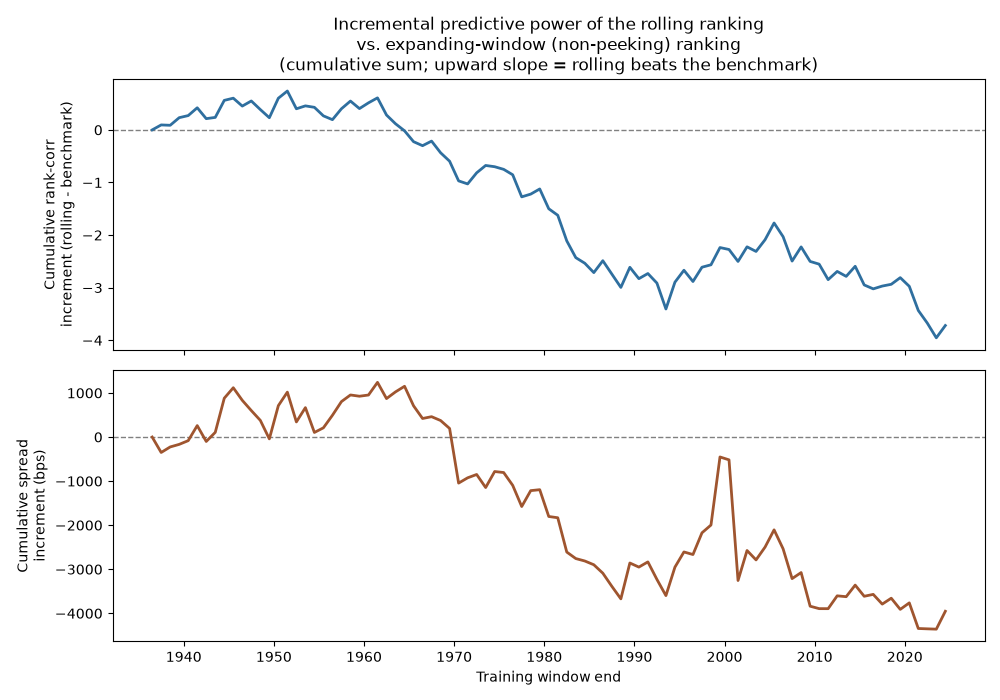
\includegraphics[width=0.82\linewidth]{incremental_rolling_vs_static_expanding_window.png}
\caption{Cumulative rolling-minus-expanding-window differential in rank
correlation (top) and quintile spread (bottom). A flat or downward path shows
the time-varying ranking does not out-predict a ranking that simply accumulates
all past data.}
\label{fig:incremental}
\end{figure}

The interpretation is unambiguous and consistent with \citet{WelchGoyal2008} and
\citet{McLeanPontiff2016}: the out-of-sample predictability documented above is
real but reflects a stable, irregular pattern of characteristic mispricing that
a fixed ranking captures at least as well; discarding data older than the rolling
window and chasing recent alpha adds estimation noise, not forecasting skill.
Claims of \emph{dynamic} forecasting ability are not supported by the data.

% =====================================================================
\section{Robustness and validation}\label{sec:robust}
% =====================================================================
\paragraph{Benchmark sensitivity (FF3 vs.\ FF5).}
On the prespecified common sample (July 1963--November 2025), FF3 and FF5
posterior ranks have Spearman correlation 0.875. \textsc{me5 bm2} moves from
rank~9 under FF3 to rank~20 under FF5, an 11-position change; FDR-supported raw
alphas move from five to three; and HAC/Wald rejects joint zero alpha under both
models. Following \citet{FamaFrench2015}, part of what looks like FF3
performance is exposure to profitability and investment dimensions absent from
FF3, confirming that alpha is benchmark-dependent.

\paragraph{Window-length sensitivity.}
Rank correlations across 60-, 120-, and 180-month windows are positive but far
from one, with top-quintile membership overlap (Jaccard) that can fall below
0.40. Window length is not a neutral tuning choice; disagreement reflects
genuine temporal instability.

\paragraph{Residual diagnostics.}
Residual normality is rejected for all 25 portfolios (Jarque--Bera), serial
independence for 16 of 25 (Ljung--Box, lag 12), and conditional
homoskedasticity for all 25 (ARCH-LM, lag 12). An IID-Gaussian error model is
not credible for these returns, which is why we rely on HAC inference and block
resampling and treat GRS as secondary. On the historical 1963--1991 anchor,
HAC/Wald rejects while GRS does not, consistent with this diagnostic evidence.

\paragraph{Independent replication.}
All coefficients and HAC standard errors reproduce independently with
\texttt{statsmodels} to a tolerance of $10^{-12}$ for all 25 portfolios, and the
qualitative $5\times5$ patterns, excess-return identity, block selection, and
weighting checks pass. Independent numerical replication is distinct from source
reconciliation: the two current-snapshot comparisons remain
\textsc{not\_comparable} (Section~\ref{sec:data}) because the local acquisition
vintage is unverified.

\paragraph{Stochastic-frontier diagnostic.}
A half-normal stochastic-frontier model \citep{AignerLovellSchmidt1977} with the
conditional-inefficiency estimator of \citet{JondrowLovellMaterovSchmidt1982} is
applied only as a residual-asymmetry diagnostic; a free intercept and a one-sided
shortfall are not separately identified, so it does not substitute for alpha. The
boundary null $\sigma_u=0$ is tested with the appropriate $50{:}50$ $\chi^2$
mixture and Benjamini--Hochberg control. Only one of 25 boundary tests survives
5\% FDR, so no general efficiency ranking is warranted.

% =====================================================================
\section{Discussion}\label{sec:discussion}
% =====================================================================
The central message is a distinction the raw forward test obscures: a
\emph{stable} cross-sectional ordering of the 25 cells carries out-of-sample
information, but the \emph{time variation} of the rolling ranking does not. This
sits naturally within the skeptical asset-pricing literature. The wide rank
intervals and the 11-position FF3-to-FF5 move echo \citet{LewellenNagelShanken2010}
and \citet{HarveyLiuZhu2016}; the fragility of the adaptive scheme relative to a
fixed ordering parallels \citet{WelchGoyal2008}; and the characteristic-based,
persistent nature of the predictable component matches \citet{McLeanPontiff2016}
and the cross-sectional emphasis of \citet{Cochrane2011}. Our result does not
contradict the finding that disciplined shrinkage and rich conditioning improve
cross-sectional pricing \citep{KozakNagelSantosh2020,GuKellyXiu2020}: those
gains come from conditioning information and regularisation, whereas we study
whether re-estimating a coarse 25-cell ranking through time adds value---and it
does not.

The most defensible use of the framework is comparative and uncertainty-aware:
estimate benchmark-relative performance, shrink noisy extremes, and report rank
uncertainty. The least defensible use is to select a single portfolio from the
point rank, or to treat the rolling ranking's apparent timing ability, as a
guaranteed future excess return.

\paragraph{Limitations.}
Returns exclude transaction costs, taxes, shorting frictions, capacity, and
market impact; the top-minus-bottom construction shorts small-growth, which is
costly and capacity-constrained in practice. The source portfolios are
value-weighted research constructions, not live investable funds, and
full-sample alphas embed later data revisions. The factor model is linear with
constant betas within each window. Posterior intervals do not fully integrate
hyperparameter uncertainty and treat the HAC covariance as known, so they are
mildly optimistic. The oracle benchmark uses look-ahead information and is an
upper bound; the expanding-window benchmark is the leakage-free comparator on
which the negative incremental verdict rests. Finally, the local input vintage
cannot currently be reconciled byte-for-byte with the public source.

% =====================================================================
\section{Conclusion}\label{sec:conclusion}
% =====================================================================
This paper provides an uncertainty-aware benchmark for the 25 Fama--French
portfolios built on a validated panel, a full joint HAC covariance, multivariate
empirical-Bayes shrinkage, multiplicity control, overlap-aware persistence
analysis, and strictly forward validation. Cross-sectional FF3 alpha variation
is present and jointly significant, but its apparent precision is substantially
reduced by partial pooling, bootstrap rank uncertainty, temporal mobility, and
benchmark sensitivity. The main contribution is the incremental forward test:
framed as a Diebold--Mariano/Giacomini--White comparison, it shows that the
positive out-of-sample quintile spread is driven by persistent characteristic
mispricing captured by a stable ordering, not by dynamic skill in the
re-estimated ranking. Future work should test whether any residual signal
survives realistic turnover and trading costs, whether additional prespecified
factors absorb the FF3 residual alphas without specification search, and whether
a decision-theoretic allocation over rank probabilities improves on hard
top-quintile selection. Any real-time claim should also await reconciliation of
the data vintage with the official source.

% =====================================================================
\appendix
\section{Reproducibility}
The reviewed environment is CPython 3.13; the deterministic bootstrap uses seed
2026. Source hashes, settings, and runtime are persisted in
\texttt{results/run\_manifest.json}. The full pipeline is
\texttt{pip install -r requirements-dev-lock.txt}; \texttt{pytest -q};
\texttt{ruff check .}; \texttt{MPLBACKEND=Agg python -m analysis.run\_all};
\texttt{python -m analysis.export\_tables};
\texttt{python reports/generate\_report.py}. The incremental test is produced
within \texttt{analysis.run\_all} and can be regenerated with
\texttt{python -m analysis.incremental\_validation --scheme all}.

% =====================================================================
% References. All entries verified against Crossref (July 2026); each carries a
% resolving DOI link. No reference is fabricated.
% =====================================================================
\begin{thebibliography}{99}

\bibitem[Aigner, Lovell, and Schmidt(1977)]{AignerLovellSchmidt1977}
Aigner, D.\ J., Lovell, C.\ A.\ K., and Schmidt, P. (1977).
Formulation and estimation of stochastic frontier production function models.
\textit{Journal of Econometrics}, 6(1), 21--37.
\href{https://doi.org/10.1016/0304-4076(77)90052-5}{https://doi.org/10.1016/0304-4076(77)90052-5}.

\bibitem[Benjamini and Hochberg(1995)]{BenjaminiHochberg1995}
Benjamini, Y., and Hochberg, Y. (1995).
Controlling the false discovery rate: a practical and powerful approach to
multiple testing.
\textit{Journal of the Royal Statistical Society: Series B}, 57(1), 289--300.
\href{https://doi.org/10.1111/j.2517-6161.1995.tb02031.x}{https://doi.org/10.1111/j.2517-6161.1995.tb02031.x}.

\bibitem[Cochrane(2011)]{Cochrane2011}
Cochrane, J.\ H. (2011).
Presidential address: discount rates.
\textit{The Journal of Finance}, 66(4), 1047--1108.
\href{https://doi.org/10.1111/j.1540-6261.2011.01671.x}{https://doi.org/10.1111/j.1540-6261.2011.01671.x}.

\bibitem[Diebold and Mariano(1995)]{DieboldMariano1995}
Diebold, F.\ X., and Mariano, R.\ S. (1995).
Comparing predictive accuracy.
\textit{Journal of Business \& Economic Statistics}, 13(3), 253--263.
\href{https://doi.org/10.1080/07350015.1995.10524599}{https://doi.org/10.1080/07350015.1995.10524599}.

\bibitem[Efron and Morris(1973)]{EfronMorris1973}
Efron, B., and Morris, C. (1973).
Stein's estimation rule and its competitors---an empirical Bayes approach.
\textit{Journal of the American Statistical Association}, 68(341), 117--130.
\href{https://doi.org/10.1080/01621459.1973.10481350}{https://doi.org/10.1080/01621459.1973.10481350}.

\bibitem[Fama and French(1993)]{FamaFrench1993}
Fama, E.\ F., and French, K.\ R. (1993).
Common risk factors in the returns on stocks and bonds.
\textit{Journal of Financial Economics}, 33(1), 3--56.
\href{https://doi.org/10.1016/0304-405X(93)90023-5}{https://doi.org/10.1016/0304-405X(93)90023-5}.

\bibitem[Fama and French(2010)]{FamaFrench2010}
Fama, E.\ F., and French, K.\ R. (2010).
Luck versus skill in the cross-section of mutual fund returns.
\textit{The Journal of Finance}, 65(5), 1915--1947.
\href{https://doi.org/10.1111/j.1540-6261.2010.01598.x}{https://doi.org/10.1111/j.1540-6261.2010.01598.x}.

\bibitem[Fama and French(2015)]{FamaFrench2015}
Fama, E.\ F., and French, K.\ R. (2015).
A five-factor asset pricing model.
\textit{Journal of Financial Economics}, 116(1), 1--22.
\href{https://doi.org/10.1016/j.jfineco.2014.10.010}{https://doi.org/10.1016/j.jfineco.2014.10.010}.

\bibitem[Fama and French(2016)]{FamaFrench2016}
Fama, E.\ F., and French, K.\ R. (2016).
Dissecting anomalies with a five-factor model.
\textit{The Review of Financial Studies}, 29(1), 69--103.
\href{https://doi.org/10.1093/rfs/hhv043}{https://doi.org/10.1093/rfs/hhv043}.

\bibitem[Giacomini and White(2006)]{GiacominiWhite2006}
Giacomini, R., and White, H. (2006).
Tests of conditional predictive ability.
\textit{Econometrica}, 74(6), 1545--1578.
\href{https://doi.org/10.1111/j.1468-0262.2006.00718.x}{https://doi.org/10.1111/j.1468-0262.2006.00718.x}.

\bibitem[Gibbons, Ross, and Shanken(1989)]{GRS1989}
Gibbons, M.\ R., Ross, S.\ A., and Shanken, J. (1989).
A test of the efficiency of a given portfolio.
\textit{Econometrica}, 57(5), 1121--1152.
\href{https://doi.org/10.2307/1913625}{https://doi.org/10.2307/1913625}.

\bibitem[Gu, Kelly, and Xiu(2020)]{GuKellyXiu2020}
Gu, S., Kelly, B., and Xiu, D. (2020).
Empirical asset pricing via machine learning.
\textit{The Review of Financial Studies}, 33(5), 2223--2273.
\href{https://doi.org/10.1093/rfs/hhaa009}{https://doi.org/10.1093/rfs/hhaa009}.

\bibitem[Harvey, Liu, and Zhu(2016)]{HarveyLiuZhu2016}
Harvey, C.\ R., Liu, Y., and Zhu, H. (2016).
$\ldots$ and the cross-section of expected returns.
\textit{The Review of Financial Studies}, 29(1), 5--68.
\href{https://doi.org/10.1093/rfs/hhv059}{https://doi.org/10.1093/rfs/hhv059}.

\bibitem[Jondrow et al.(1982)]{JondrowLovellMaterovSchmidt1982}
Jondrow, J., Lovell, C.\ A.\ K., Materov, I.\ S., and Schmidt, P. (1982).
On the estimation of technical inefficiency in the stochastic frontier
production function model.
\textit{Journal of Econometrics}, 19(2--3), 233--238.
\href{https://doi.org/10.1016/0304-4076(82)90004-5}{https://doi.org/10.1016/0304-4076(82)90004-5}.

\bibitem[Jorion(1986)]{Jorion1986}
Jorion, P. (1986).
Bayes--Stein estimation for portfolio analysis.
\textit{The Journal of Financial and Quantitative Analysis}, 21(3), 279--292.
\href{https://doi.org/10.2307/2331042}{https://doi.org/10.2307/2331042}.

\bibitem[Kosowski et al.(2006)]{KosowskiTimmermannWermersWhite2006}
Kosowski, R., Timmermann, A., Wermers, R., and White, H. (2006).
Can mutual fund ``stars'' really pick stocks? New evidence from a bootstrap
analysis.
\textit{The Journal of Finance}, 61(6), 2551--2595.
\href{https://doi.org/10.1111/j.1540-6261.2006.01015.x}{https://doi.org/10.1111/j.1540-6261.2006.01015.x}.

\bibitem[Kozak, Nagel, and Santosh(2020)]{KozakNagelSantosh2020}
Kozak, S., Nagel, S., and Santosh, S. (2020).
Shrinking the cross-section.
\textit{Journal of Financial Economics}, 135(2), 271--292.
\href{https://doi.org/10.1016/j.jfineco.2019.06.008}{https://doi.org/10.1016/j.jfineco.2019.06.008}.

\bibitem[K\"unsch(1989)]{Kunsch1989}
K\"unsch, H.\ R. (1989).
The jackknife and the bootstrap for general stationary observations.
\textit{The Annals of Statistics}, 17(3), 1217--1241.
\href{https://doi.org/10.1214/aos/1176347265}{https://doi.org/10.1214/aos/1176347265}.

\bibitem[Lewellen, Nagel, and Shanken(2010)]{LewellenNagelShanken2010}
Lewellen, J., Nagel, S., and Shanken, J. (2010).
A skeptical appraisal of asset pricing tests.
\textit{Journal of Financial Economics}, 96(2), 175--194.
\href{https://doi.org/10.1016/j.jfineco.2009.09.001}{https://doi.org/10.1016/j.jfineco.2009.09.001}.

\bibitem[McLean and Pontiff(2016)]{McLeanPontiff2016}
McLean, R.\ D., and Pontiff, J. (2016).
Does academic research destroy stock return predictability?
\textit{The Journal of Finance}, 71(1), 5--32.
\href{https://doi.org/10.1111/jofi.12365}{https://doi.org/10.1111/jofi.12365}.

\bibitem[Newey and West(1987)]{NeweyWest1987}
Newey, W.\ K., and West, K.\ D. (1987).
A simple, positive semi-definite, heteroskedasticity and autocorrelation
consistent covariance matrix.
\textit{Econometrica}, 55(3), 703--708.
\href{https://doi.org/10.2307/1913610}{https://doi.org/10.2307/1913610}.

\bibitem[Newey and West(1994)]{NeweyWest1994}
Newey, W.\ K., and West, K.\ D. (1994).
Automatic lag selection in covariance matrix estimation.
\textit{The Review of Economic Studies}, 61(4), 631--653.
\href{https://doi.org/10.2307/2297912}{https://doi.org/10.2307/2297912}.

\bibitem[Politis and Romano(1994)]{PolitisRomano1994}
Politis, D.\ N., and Romano, J.\ P. (1994).
The stationary bootstrap.
\textit{Journal of the American Statistical Association}, 89(428), 1303--1313.
\href{https://doi.org/10.1080/01621459.1994.10476870}{https://doi.org/10.1080/01621459.1994.10476870}.

\bibitem[Welch and Goyal(2008)]{WelchGoyal2008}
Welch, I., and Goyal, A. (2008).
A comprehensive look at the empirical performance of equity premium prediction.
\textit{The Review of Financial Studies}, 21(4), 1455--1508.
\href{https://doi.org/10.1093/rfs/hhm014}{https://doi.org/10.1093/rfs/hhm014}.

\end{thebibliography}

\end{document}
